\documentclass{article}
\title{Theo 1 Abgabe 2}
\author{Nick Daiber}
\usepackage{amsmath}
\usepackage{amssymb}
\usepackage{amsfonts}
\usepackage{tikz}
\usetikzlibrary{automata,positioning}

\begin{document}
\maketitle
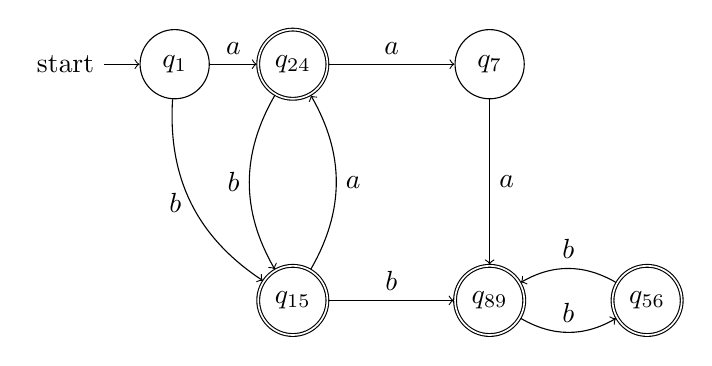
\begin{tikzpicture}[align=center,node distance=2cm]
    \node[state, initial] at (0, 3) (q1) {$q_1$};
    \node[state] at (4, 3) (q7) {$q_7$};
    \node[state, accepting] at (1.5, 0) (q15) {$q_{15}$};
    \node[state, accepting] at (1.5, 3) (q24) {$q_{24}$};
    \node[state, accepting] at (4, 0) (q89) {$q_{89}$};
    \node[state, accepting] at (6, 0) (q56) {$q_{56}$};
    \draw[->]
    (q1) edge[above] node{$a$} (q24)
    (q1) edge[left, bend right] node{$b$} (q15)
    (q7) edge[right] node{$a$} (q89)
    (q24) edge[above] node{$a$} (q7)
    (q24) edge[left, bend right] node{$b$} (q15)

    (q15) edge[right, bend right] node{$a$} (q24)
    (q15) edge[above] node{$b$} (q89)
    (q89) edge[above, bend right] node{$b$} (q56)
    (q56) edge[above, bend right] node{$b$} (q89)

    %(A) edge[above] node{$a$} (B)
    %(B) edge[above] node{$a$} (C);
    ;
\end{tikzpicture}

\end{document}